\documentclass{anstrans}
%%%%%%%%%%%%%%%%%%%%%%%%%%%%%%%%%%%
\title{Extension of the entropy viscosity method to the $1$-D Seven-Equation Model}
\author{Marc O. Delchini$^{*}$, Jean C. Ragusa$^{*}$, Ray A. Berry$^\dagger$}

\institute{
$^{*}$Department of Nuclear Engineering, Texas A\&M University, 
$^\dagger$Idaho National Laboratory
}

\email{delchmo@tamu.edu \and jean.ragusa@.tamu.edu \and ray.berry@inl.gov}

% Optional disclaimer: remove this command to hide
%\disclaimer{Notice: This manuscript is a work of fiction. Any resemblance to actual articles, living or dead, is purely coincidental.}

%%%% packages and definitions (optional)
\usepackage{graphicx} % allows inclusion of graphics
\usepackage{booktabs} % nice rules (thick lines) for tables
\usepackage{microtype} % improves typography for PDF
%\usepackage{subfigure}
\usepackage{subcaption}
\usepackage{float}


\renewcommand{\div}{\vec{\nabla}\! \cdot \!}
\newcommand{\grad}{\vec{\nabla}}
\newcommand{\divv}[1]{\vec{\nabla}^{#1}\! \cdot \!}
\newcommand{\gradd}[1]{\vec{\nabla}^{#1}}
% latex shortcuts
\newcommand{\bea}{\begin{eqnarray}}
\newcommand{\eea}{\end{eqnarray}}
\newcommand{\be}{\begin{equation}}
\newcommand{\ee}{\end{equation}}
\newcommand{\bal}{\begin{align}}
\newcommand{\eali}{\end{align}}
\newcommand{\bi}{\begin{itemize}}
\newcommand{\ei}{\end{itemize}}
\newcommand{\ben}{\begin{enumerate}}
\newcommand{\een}{\end{enumerate}}
% DGFEM commands
\newcommand{\jmp}[1]{[\![#1]\!]}                     % jump
\newcommand{\mvl}[1]{\{\!\!\{#1\}\!\!\}}             % mean value
\newcommand{\keff}{\ensuremath{k_{\textit{eff}}}\xspace}
% shortcut for domain notation
\newcommand{\D}{\mathcal{D}}
% vector shortcuts
\newcommand{\vo}{\vec{\Omega}}
\newcommand{\vr}{\vec{r}}
\newcommand{\vn}{\vec{n}}
\newcommand{\vnk}{\vec{\mathbf{n}}}
\newcommand{\vj}{\vec{J}}
\newcommand{\eig}[1]{\| #1 \|_2}

\newcommand{\EI}{\mathcal{E}_h^i}
\newcommand{\ED}{\mathcal{E}_h^{\partial \D^d}}
\newcommand{\EN}{\mathcal{E}_h^{\partial \D^n}}
\newcommand{\ER}{\mathcal{E}_h^{\partial \D^r}}
\newcommand{\reg}{\textit{reg}}

\newcommand{\norm}{\textrm{norm}}
\renewcommand{\Re}{\textrm{Re}}
\newcommand{\Pe}{\textrm{P\'e}}
\renewcommand{\Pr}{\textrm{Pr}}

\newcommand{\resi}{R_e}
%\newcommand{\resinew}{\tilde{D}_e}
\newcommand{\resinew}{\widetilde{\resi}}
\newcommand{\matder}[1]{\frac{\textrm{D} #1}{\textrm{D} t}}


% extra space
\newcommand{\qq}{\quad\quad}
% common reference commands
\newcommand{\eqt}[1]{Eq.~(\ref{#1})}                     % equation
\newcommand{\fig}[1]{Fig.~\ref{#1}}                      % figure
\newcommand{\tbl}[1]{Table~\ref{#1}}                     % table
\newcommand{\sct}[1]{Section~\ref{#1}}                   % section
\newcommand{\app}[1]{Appendix~\ref{#1}}                   % appendix

\newcommand\br{\mathbf{r}}
%\newcommand{\tf}{\varphi}
\newcommand{\tf}{b}


\begin{document}
%%%%%%%%%%%%%%%%%%%%%%%%%%%%%%%%%%%%%%%%%%%%%%%%%%%%%%%%%%%%%%%%%%%%%%%%%%%%%%%%
\section{Introduction}
%
We extend the entropy viscosity method, proposed by Guermond et al. \cite{jlg1, jlg2}
to the well-posed $1$-D seven-equation model \cite{DEM}. The entropy viscosity technique is a viscous regularization technique
that satisfies the entropy minimum principle; adequate dissipation terms (viscous fluxes)
are added to the governing laws while ensuring the entropy minimum principle still holds.
Viscosity coefficients modulates the magnitude of the added dissipation such that it is
large in shock regions and vanishingly small elsewhere. The entropy viscosity coefficients
are taken proportional to the entropy production while, at the same time, being bounded
from above by a first-order viscosity coefficient that reduces the spatial discretization
to be similar to a first-order Godunov scheme (the latter being known to be overly dissipative but
monotone \cite{toro}). Hence, entropy production in shocks will result in large viscosity  
coefficients and thus will avoid spurious oscillations. 

The entropy method is independent of the type of spatial discretization (finite volume,
continuous or discontinuous finite elements, ...) and thus can be applied ubiquitously. 
The results presented in this summary were obtained with RELAP-7, the next-generation 
reactor system code build upon the MOOSE multiphysics framework
\cite{moose} that uses \emph{Galerkin Continuous Finite Element Method}.

In this summary, the $1$-D seven-equation model is recalled along with the dissipative terms used 
in the entropy method. Definition of the viscosity coefficients is also given and numerical 
results are presented for a $1$-D pipe with wall-heat transfer.
%
%%%%%%%%%%%%%%%%%%%%%%%%%%%%%%%%%%%%%%%%%%%%%%%%%%%%%%%%%%%%%%%%%%%%%%%%%%%%%%%%
\section{Theory}
%
We recall the $1$-D seven-equation model for two phases $k$ and $j$ with viscous regularization (inside boxes) based on the entropy-viscosity 
method (the equations are given for the phase $k$ and can be obtained for the phase $j$ by simply substituing $k$ by $j$ and vice versa):
\begin{subequations}
\label{eq:euler_visc}
%
\begin{equation}\label{eq:vf_eq}
  \frac{\partial \alpha_{k} A}{\partial t} + u_{int} A \frac{\partial \alpha_{k}}{\partial x}
  = A \mu (p_{k} - p_{j}) - \frac{\Gamma A_{int} A}{\rho_{int}} + \boxed{\frac{\partial }{\partial x} \left( A l_k  \right)}
\end{equation}
%
\begin{eqnarray}
  \frac{\partial \left( \alpha \rho \right)_{k} A}{\partial t}
  + \frac{\partial \left( \alpha \rho u \right)_{k} A}{\partial x}
  = - \Gamma A_{int} A
   + \boxed{\frac{\partial }{\partial x} \left( A f_k \right)}
\end{eqnarray}
%
\begin{eqnarray}
 && \frac{\partial \left( \alpha \rho u \right)_{k} A}{\partial t}
  + \frac{\partial \alpha_{k} A \left( \rho u^2 + p \right)_{k} }{\partial x}   = p_{int} A \frac{\partial \alpha_{k}}{\partial x} \nonumber \\
 &&+ p_{k} \alpha_{k} \frac{\partial A}{\partial x}
  + A \lambda (u_{j} - u_{k}) - \Gamma A_{int} u_{int} A - \nonumber \\
  &&F_{\text{wall friction}, k} - F_{\text{friction}, j}
  + \left( \alpha \rho \right)_{k} A \vec{g} \cdot \vec{n}_{axis} \nonumber \\
 && + \boxed{\frac{\partial }{\partial x} \left[ A \left( g_k + u_k f_k \right) \right] }
\end{eqnarray}
%
\begin{eqnarray}
 &&\frac{\partial \left( \alpha \rho E \right)_{k} A}{\partial t}
  + \frac{\partial \alpha_{k} u_{k} A \left( \rho E + p \right)_{k}}{\partial x}
  = p_{int} u_{int} A \frac{\partial \alpha_{k}}{\partial x} 
  \nonumber \\
  &&- \bar{p}_{int} A \mu (p_{k} - p_{j})+ \bar{u}_{int} A \lambda (u_{j} - u_{k})
  \nonumber \\
  &&+ \Gamma A_{int} \left( \frac{p_{int}}{\rho_{int}} - H_{k, int} \right) A
  + Q_{int, k} + Q_{\text{wall}, k} \nonumber \\ 
 && + \boxed{\frac{\partial }{\partial x} \left[ A \left( h_k + u_k g_k - \frac{u_k^2}{2}f_k + \rho_k e_k l_k\right) \right] }
\end{eqnarray}
%
\end{subequations}
where the dissipative terms have the following definition:
\begin{subequations}
%
\begin{equation}
  l_k = \beta_k \partial_x \alpha_k 
\end{equation}
%  
\begin{equation}
  f_k = \alpha_k \kappa_k \partial_x \rho_k + \rho_k l_k 
\end{equation}
%  
\begin{equation}
  g_k = \alpha_k \mu_k \rho_k \partial_x u_k 
\end{equation}  
%
\begin{equation}
  h_k =  \alpha_k \kappa_k \partial_x \left( \rho_k e_k \right)
 \end{equation}
%
\end{subequations}
The notation is standard: $\alpha_k$, $\rho_k$, $(\rho \vec{u})_k$ and $(\rho E)_k$ are the volume fraction, the density, the momentum and the total energy for phase $k$, respectively, and will be referred to as the conservative variables. $\vec{u}_k$ is the fluid velocity for phase $k$ and its specific internal energy is denoted by $e_k=E_k-\tfrac{u^2_k}{2}$. The area $A$ is a given and can be spatial-dependent. The stiffened gas equation of state \cite{SGEOS} is used to compute the pressure $P_k$. Definitions of the interfacial variables denoted by the subscript $int$ and the source terms (mass transfer ($\Gamma$), friction and heat source) can be found in \cite{berry}. $\beta_{e,k}$, $\kappa_{e,k}$ and $\mu_{e,k}$ are distinct positive viscosity coefficients and are based on the local entropy production in phase $k$. The definition of the coefficients $\mu_{e,k}$ and $\kappa_{e,k}$ is identical to the one used for the multi-D Euler equations \cite{marco_inl_report} and yield well-scaled dissipative terms in the low-Mach regime \cite{LowMach1, LowMach2, LowMach3}:
%
\begin{subequations}
\label{eq:ent_visc_coeff2}
\begin{equation}
\mu^K_{e,k}(\vec{r}_q,t) =  h_K^2 \frac{| \resinew^K(\vec{r}_q,t) |}{M \rho \|\vec{u}\|^2 + (1-M) \rho c^2}  
\end{equation}
\begin{equation}
\kappa^K_{e,k}(\vec{r}_q,t) = Pr_k \, \mu^K_e(\vec{r}_q,t)
\end{equation}
\end{subequations}
%
where $c_k$ is the phase speed of sound and the weighting factor is the local Mach number, $M_k=\|\vec{u_k}\|/c_k$. $K$ is a given element of the mesh, and $\vec{r}_q$ is a quadrature point location within cell $K$. $\Pr_k$ is the Prandtl number; see \cite{jlg1} for additional details. The entropy residual is denoted by $\resinew$ and its definition is recalled in \eqt{eq:ent2_res}.  
%
\begin{equation}
\label{eq:ent2_res}
\resinew(\vec{r_q},t) := \left( \matder{P_k} - c^2_k \matder{\rho_k} \right) \propto \partial_t s_k + \vec{u} \cdot \grad s_k = \matder{s_k},
\end{equation} 
%
where $s_k$ is the phase entropy, function of the density $\rho_k$ and the internal energy $e_k$. Proof of \eqt{eq:ent2_res} can be found in \cite{marco_inl_report}.

The approach to define the viscosity coefficient $\beta_k$ is similar to the logic followed for hyperbolic scalar equations \cite{jlg1, jlg2}: an entropy equation can be derived from the volume fraction equation (\eqt{eq:vf_eq}) and used in the definition of the coefficient $\beta_k$. Following the work by Guermond et al. \cite{jlg1, jlg2}, it yields:
%
\begin{subequations}
\begin{equation}
\beta^K_{e,k}(\vec{r}_q,t) =  h_K^2 \frac{| R_{\alpha,k}^K(\vec{r}_q,t) |}{\alpha_k},
\end{equation}
where the entropy residual associated to the volume fraction equation, \eqt{eq:vf_eq}, is
\begin{equation}
\label{eq:beta_def}
R_{\alpha,k}^K(\vec{r}_q,t) =   \frac{1}{2} \left( \frac{\partial \alpha_{k}^2}{\partial t} + u_{int} \frac{\partial \alpha_{k}^2}{\partial x} \right).
\end{equation} 
\end{subequations}
% 
where $s_{\alpha,k} = \alpha_k^2/2$ can be seen at the entropy function associated to the volume fraction equation of phase $k$.
%%%%%%%%%%%%%%%%%%%%%%%%%%%%%%%%%%%%%%%%%%%%%%%%%%%%%%%%%%%%%%%%%%%%%%%%%%%%%%%%
\section{Results and Analysis}

The Euler equation with viscous stabilization are discretized with {\it continuous} finite elements in space and BDF2 in time using MOOSE. The resulting nonlinear system of equations at each time step is solved using a Jacobian-free Newton Krylov technique. We present results a 2D flow over a circular hump . such problems are often employ to test the ability of a numerical scheme used in compressible  flow solvers to resolve low-Mach flows (i.e., in the incompressible limit)
\cite{LowMach1}. 

The results are shown in \fig{fig:2d_hump_mach_0p7}, \fig{fig:2d_hump_mach_0p01}, \fig{fig:2d_hump_mach_0p0001} and \fig{fig:2d_hump_mach_0p0000001} for inlet Mach numbers $M_{\infty}=0.7$, $M_{\infty}=0.01$, $M_{\infty}=10^{-4}$ and $M_{\infty}=10^{-7}$, respectively. It is expected that, within the low-Mach number range, the solution does not depend on the Mach number and is self-similar. The results showed in \fig{fig:2d_hump_mach_0p01}, \fig{fig:2d_hump_mach_0p0001} and \fig{fig:2d_hump_mach_0p0000001} correspond to the low-Mach regime. The iso-Mach lines are drawn ranging from the minimum and the maximum values (provided in each legend) using 50 equally-spaced intervals. The steady-state solution is symmetric and does not depend on the value of the inlet Mach number, as expected in the incompressible limit. 
%
For a flow at $M=0.7$, the compressible effects become more important and shock can form. An uniform grid of $3352$ $Q_1$ elements was used to obtain the numerical solution for Mach numbers below $M_{\infty}=0.01$. A once-refined mesh was employed for the $M_{\infty}=0.7$ simulation in order to better resolve the shock. A $CFL$ of 20 was employed and the simulations were run until steady state. 
%
In \fig{fig:2d_hump_mach_0p7}, the steady-state numerical solution develops a shock: the compressibility effect are no longer negligible. The iso-Mach lines are also plotted with $50$ intervals and range from $0.4$ to $1.6$. The shock is well resolved and does not display any instabilities or spurious oscillations. 
%
\begin{figure}[H]
        \centering
        \begin{subfigure}[b]{0.5\textwidth}
                \centering
                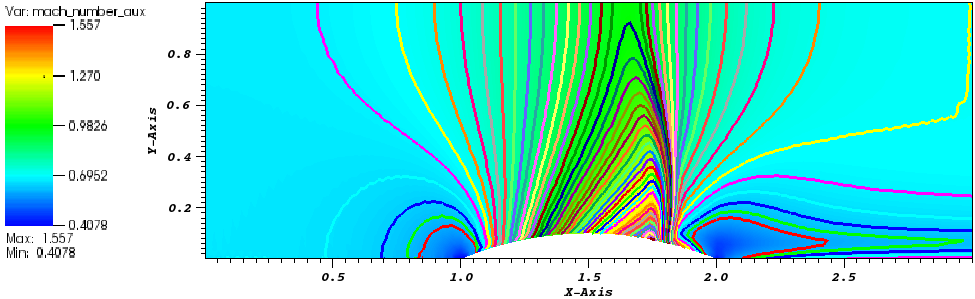
\includegraphics[width=\textwidth]{Hump2D_mach_0p7.png}
                \caption{Mach $0.7$}
                \label{fig:2d_hump_mach_0p7}
        \end{subfigure}%

        \begin{subfigure}[b]{0.5\textwidth}
                \centering
                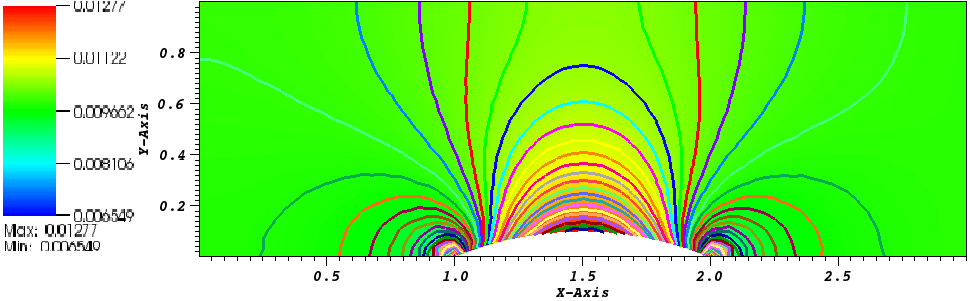
\includegraphics[width=\textwidth]{Hump2D_mach_0p01.png}
                \caption{Mach $10^{-2}$}
                \label{fig:2d_hump_mach_0p01}
        \end{subfigure}%
        
        \begin{subfigure}[b]{0.495\textwidth}
                \centering
                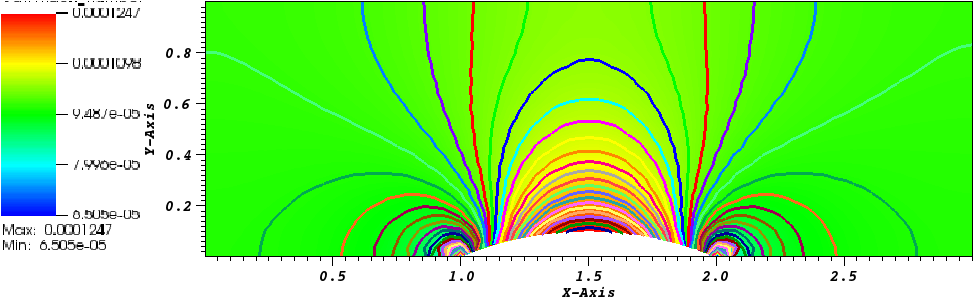
\includegraphics[width=\textwidth]{Hump2D_mach_1em4.png}
                \caption{Mach $10^{-5}$}
                \label{fig:2d_hump_mach_0p0001}
        \end{subfigure}

        \begin{subfigure}[b]{0.495\textwidth}
                \centering
                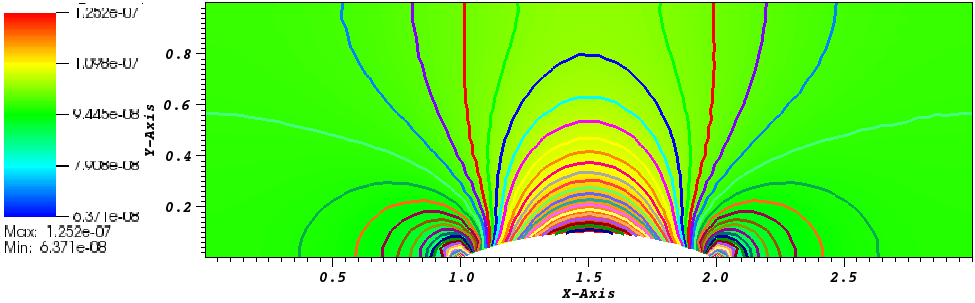
\includegraphics[width=\textwidth]{Hump2D_mach_1em7.png}
                \caption{Mach $10^{-7}$}
                \label{fig:2d_hump_mach_0p0000001}
        \end{subfigure}
        \caption{Iso-Mach lines for a 2-D flow over a circular bump (steady-state solution).}
				\label{fig:2d_hump}
\end{figure}
%
The results presented in \fig{fig:2d_hump} were obtained with the new definitions of the viscosity coefficients and illustrate the ability of the entropy viscosity method to correctly simulate several types of flows (subsonic and transonic flows) without tuning parameters. 


%%%%%%%%%%%%%%%%%%%%%%%%%%%%%%%%%%%%%%%%%%%%%%%%%%%%%%%%%%%%%%%%%%%%%%%%%%%%%%%%
\section{Conclusions}

We have presented an extension of the entropy viscosity method for low-Mach flows. In the future, we plan on adding heat generation, gravity, and friction terms. Another possible extension of this work (reported in these proceedings) deals with applying the entropy viscosity method to a 7-equation two-phase flow model. These steps will further contribute to the assessment of the stabilization technique for reactor flows.


%%%%%%%%%%%%%%%%%%%%%%%%%%%%%%%%%%%%%%%%%%%%%%%%%%%%%%%%%%%%%%%%%%%%%%%%%%%%%%%%
%\appendix
%\section{Appendix}

%%%%%%%%%%%%%%%%%%%%%%%%%%%%%%%%%%%%%%%%%%%%%%%%%%%%%%%%%%%%%%%%%%%%%%%%%%%%%%%%
%\section{Acknowledgments}
%This material is based upon work supported by the Department of Energy Rickover Fellowship Program in Nuclear Engineering.

%%%%%%%%%%%%%%%%%%%%%%%%%%%%%%%%%%%%%%%%%%%%%%%%%%%%%%%%%%%%%%%%%%%%%%%%%%%%%%%%
\bibliographystyle{ans}
\bibliography{bibliography}

\end{document}

